% ============================================================================
%  Oral Adiabatic Decompression Fog (OADF):
%  A Thermodynamic and Aerosol-Physics Analysis of Visible Vapor
%  Condensation in the Human Buccal Cavity Under Rapid Decompression
%
%  Document class: article (single-column research paper)
%  Compilation:    pdflatex → pdflatex (twice for cross-refs)
%                  No external bibliography tool required.
%  Engine:         pdfLaTeX or LuaLaTeX (TeX Live 2020+ recommended)
% ============================================================================

\documentclass[11pt,a4paper]{article}

% ---------- Encoding & fonts ----------
\usepackage[T1]{fontenc}
\usepackage[utf8]{inputenc}
\usepackage{lmodern}
\usepackage{microtype}
\usepackage{textcomp}

% ---------- Page geometry ----------
\usepackage[a4paper,
            top=2.5cm, bottom=2.5cm,
            left=2.7cm, right=2.7cm,
            headheight=16pt,
            footskip=1.2cm]{geometry}

% ---------- Math ----------
\usepackage{amsmath,amssymb,amsthm,mathtools}
\usepackage{bm}
\usepackage{physics}
\usepackage[version=4]{mhchem}
\usepackage{siunitx}
\sisetup{detect-all,
         per-mode=symbol,
         range-units=single,
         range-phrase=\,\text{--}\,,
         separate-uncertainty=true}

% ---------- Graphics & diagrams ----------
\usepackage{graphicx}
\usepackage{tikz}
\usetikzlibrary{arrows.meta,calc,decorations.pathmorphing,patterns,positioning,shadings,shapes.geometric,backgrounds}
\usepackage{pgfplots}
\pgfplotsset{compat=1.18}

% ---------- Tables ----------
\usepackage{booktabs}
\usepackage{array}
\usepackage{tabularx}
\usepackage{multirow}

% ---------- Cross-references, color, hyperlinks ----------
\usepackage{xcolor}
\usepackage[round,authoryear]{natbib}
\bibpunct{(}{)}{;}{a}{,}{,}
\definecolor{linkcolor}{HTML}{1F3A5F}
\definecolor{citecolor}{HTML}{6B4423}
\definecolor{urlcolor}{HTML}{1F3A5F}
\definecolor{accent}{HTML}{8B6F2E}
\definecolor{rule}{HTML}{2F3E4E}
\usepackage[colorlinks=true,
            linkcolor=linkcolor,
            citecolor=citecolor,
            urlcolor=urlcolor,
            breaklinks=true,
            pdftitle={Oral Adiabatic Decompression Fog (OADF)},
            pdfauthor={LiranOG},
            pdfkeywords={adiabatic expansion; cloud condensation nuclei; Wilson cloud chamber; supersaturation; bioaerosol; Köhler theory}]{hyperref}

% ---------- Section formatting ----------
\usepackage{titlesec}
\titleformat{\section}
  {\Large\bfseries\sffamily\color{linkcolor}}
  {\thesection.}{0.7em}{}
\titleformat{\subsection}
  {\large\bfseries\sffamily\color{linkcolor!85!black}}
  {\thesubsection.}{0.6em}{}
\titleformat{\subsubsection}
  {\normalsize\bfseries\sffamily}
  {\thesubsubsection.}{0.5em}{}
\titlespacing*{\section}{0pt}{2.0ex plus 1ex minus .2ex}{1.2ex plus .2ex}
\titlespacing*{\subsection}{0pt}{1.6ex plus 1ex minus .2ex}{1.0ex plus .2ex}

% ---------- Captions ----------
\usepackage{caption}
\captionsetup{font={small},labelfont={bf,sf,color=linkcolor},labelsep=period,justification=justified,singlelinecheck=false}

% ---------- Headers / footers ----------
\usepackage{fancyhdr}
\pagestyle{fancy}
\fancyhf{}
\fancyhead[L]{\small\textsf{Oral Adiabatic Decompression Fog}}
\fancyhead[R]{\small\textsf{\thepage}}
\renewcommand{\headrulewidth}{0.4pt}
\renewcommand{\headrule}{\hbox to\headwidth{\color{rule}\leaders\hrule height \headrulewidth\hfill}}

% ---------- Misc ----------
\usepackage{enumitem}
\setlist[itemize]{leftmargin=*,topsep=2pt,itemsep=2pt,parsep=0pt}
\setlist[enumerate]{leftmargin=*,topsep=2pt,itemsep=2pt,parsep=0pt}

\usepackage[normalem]{ulem}
\usepackage{epigraph}
\setlength{\epigraphwidth}{0.55\textwidth}
\renewcommand{\textflush}{flushright}
\renewcommand{\epigraphrule}{0pt}

\usepackage{tcolorbox}
\tcbuselibrary{breakable,skins}

\newtcolorbox{keypoint}[1][]{
  enhanced, breakable, sharp corners,
  colback=accent!7, colframe=accent!50!black,
  boxrule=0.5pt, left=10pt, right=10pt, top=8pt, bottom=8pt,
  fonttitle=\bfseries\sffamily,
  title=#1
}

% ---------- Math operators / commands ----------
\DeclareMathOperator{\sgn}{sgn}
\newcommand{\Sat}{S_{\text{sat}}}
\newcommand{\pwsat}{p_{w,\text{sat}}}
\newcommand{\Tref}{T_{\text{ref}}}
\renewcommand{\vec}[1]{\mathbf{#1}}

% ---------- Theorem styles ----------
\theoremstyle{definition}
\newtheorem{definition}{Definition}[section]
\newtheorem{remark}{Remark}[section]

\theoremstyle{plain}
\newtheorem{proposition}{Proposition}[section]

% =========================================================================
%  TITLE BLOCK
% =========================================================================

\title{\vspace{-1.2cm}
\sffamily\bfseries
Oral Adiabatic Decompression Fog (OADF):\\[2pt]
\large\mdseries\itshape
A Thermodynamic and Aerosol-Physics Analysis of Visible Vapor Condensation in the Human Buccal Cavity Under Rapid Decompression
\vspace{-0.2cm}
}

\author{%
\textbf{Liran~M.~Schwartz}\thanks{Independent Researcher. ORCID: \href{https://orcid.org/0009-0008-8035-1308}{0009-0008-8035-1308}. Correspondence: \texttt{scliran9@gmail.com}. Zenodo: \href{https://doi.org/10.5281/zenodo.20309015}{10.5281/zenodo.20309015}.\\[1pt]
\small\itshape Independent Research\\
\small\itshape Haifa, Israel
}

\date{\small Working draft \textperiodcentered{} \today}

% =========================================================================
%  DOCUMENT BEGIN
% =========================================================================

\begin{document}
\maketitle
\thispagestyle{empty}

% ---------- Abstract ----------
\begin{center}
\begin{minipage}{0.92\textwidth}
\small
\noindent\textbf{Abstract.}\quad
We provide a unified thermodynamic and aerosol-microphysical analysis of a familiar but undocumented everyday phenomenon: the brief, visible white plume produced when an individual seals the buccal cavity, performs mechanical compression of the trapped gas (typically via repeated tongue-palate clicks and cheek/diaphragm action), and then rapidly opens the oral aperture. We argue that this phenomenon, here proposed under the descriptive name \emph{Oral Adiabatic Decompression Fog} (OADF), constitutes a low-cost, biologically self-supplying analogue of the Wilson expansion cloud chamber. The buccal cavity satisfies three independently necessary preconditions for visible condensation under rapid decompression: (i) near-saturated water-vapor humidity at body temperature ($T_0 \approx \SI{310}{\kelvin}$, $\mathrm{RH} \approx 100\%$); (ii) a transient overpressure achievable by voluntary musculature ($\Delta P \sim \SIrange{5}{15}{\kilo\pascal}$); and (iii) a high background concentration of soluble bio-aerosol cloud condensation nuclei (CCN) originating from saliva atomization. We derive the governing relations from the Poisson adiabatic equation, the Clausius–Clapeyron equation, and Köhler theory, present a closed-form expression for the post-expansion supersaturation ratio, and provide order-of-magnitude estimates for the resulting droplet number density, droplet size, and condensed water mass. For a representative compression of $P_2/P_1 = 1.10$, the model predicts a temperature drop of $\Delta T \approx \SI{8.4}{\kelvin}$, a saturation ratio of $S \approx 1.46$ (\SI{46}{\percent} supersaturation), and an excess condensed water content of $\sim\SI{12.9}{\gram\per\cubic\meter}$ in the emerging plume — values consistent with the qualitative optical density routinely observed. We position OADF within the broader taxonomy of expansion-condensation phenomena (champagne cork plumes, transonic-flow Prandtl–Glauert condensation, atmospheric cloud formation), propose an experimental protocol to characterize OADF quantitatively, and identify open questions concerning the role of organic surfactants in saliva-derived CCN. The phenomenon merits no claim of physical novelty; its scientific value is pedagogical and aerosol-biological, with potential applications in physics education and in studies of respiratory bioaerosol generation.

\vspace{0.5em}
\noindent\textbf{Keywords:}\quad
adiabatic expansion \textperiodcentered{} cloud condensation nuclei \textperiodcentered{} Wilson cloud chamber \textperiodcentered{} supersaturation \textperiodcentered{} bioaerosol \textperiodcentered{} Köhler theory \textperiodcentered{} respiratory physics \textperiodcentered{} expansion-condensation fog

\vspace{0.4em}
\noindent\textbf{PACS:}\quad 47.55.dd \textperiodcentered{} 92.60.Mt \textperiodcentered{} 87.85.gj\\
\noindent\textbf{Classification (MSC2020):}\quad 76T10 \textperiodcentered{} 80A22 \textperiodcentered{} 92C30
\end{minipage}
\end{center}

\vspace{0.6em}
\noindent\hrulefill
\vspace{0.6em}

\tableofcontents
\vspace{1em}
\noindent\hrulefill

\newpage

% =========================================================================
\section{Introduction}
% =========================================================================

\epigraph{\itshape ``When air saturated with water vapour is suddenly cooled by an adiabatic expansion, it becomes supersaturated. In this condition, condensation into droplets will occur, provided there are nuclei present.''}{--- C.~T.~R. Wilson, Nobel Lecture, 1927}

\subsection{The phenomenon}
\label{sec:phenomenon}

A child, sealing the lips with one hand, repeatedly clicks the tongue against the hard palate to drive air into the closed oral cavity. After a few seconds of mechanical pressurization, the lips are released; a brief, visible, optically dense white plume emerges, persisting for $\sim\!1\text{--}3$ seconds before dispersing. The plume is colloquially described as ``smoke,'' although nothing has been combusted and no solid aerosol of macroscopic origin is present. Anecdotal evidence places the trick within the common repertoire of childhood play across multiple cultures and decades; we have, however, been unable to identify a dedicated published treatment of the phenomenon in either the atmospheric, respiratory, or pedagogical physics literatures.

The phenomenon is qualitatively familiar to anyone who has performed it, yet it occupies a curious gap in the technical record. It is universally accessible, optically striking, and physically rich — combining classical thermodynamics, vapor-phase microphysics, and bio-aerosol generation in a single sub-second event. We argue here that it merits formal description, that it can be placed cleanly within an established theoretical framework, and that the same framework yields immediate quantitative predictions that any properly equipped laboratory could test in an afternoon.

\subsection{Proposed nomenclature}
\label{sec:naming}

We propose the descriptive name \emph{Oral Adiabatic Decompression Fog} (\textbf{OADF}). The term is intended to:
\begin{enumerate}
  \item \textbf{Localize} the phenomenon to the buccal cavity (\emph{oral}), distinguishing it from cognate phenomena occurring in mechanical chambers (Wilson), pressurized vessels (champagne), and gas-dynamic flows (transonic condensation cones);
  \item \textbf{Identify the driving thermodynamic process} (\emph{adiabatic decompression}), distinguishing it from \emph{mixing-fog} phenomena such as exhaled-breath condensation in cold ambient air, whose mechanism differs fundamentally (cf.~Sec.~\ref{sec:mixingfog});
  \item \textbf{Characterize the visible product} as a fog of condensed liquid-water droplets, in continuity with established usage in atmospheric science.
\end{enumerate}
We make no claim of priority on the underlying physics, which has been understood since the work of \citet{Wilson1897,Wilson1911} and \citet{Koehler1936}. The proposal is solely terminological: a name for the specific instance.

\subsection{Contribution}
\label{sec:contribution}

The present paper provides four contributions:
\begin{enumerate}
  \item A complete thermodynamic decomposition of the OADF event into four sequential phases (saturation, compression, adiabatic decompression, condensation), with explicit governing equations for each phase (Sec.~\ref{sec:framework}).
  \item A closed-form expression, derived from the Poisson adiabatic relation combined with the Clausius–Clapeyron equation, for the post-expansion saturation ratio $S$ as a function of the compression ratio $\Pi = P_2/P_1$ and initial temperature $T_0$ (Sec.~\ref{sec:formalization}, Eq.~\ref{eq:S-final}).
  \item An order-of-magnitude numerical estimation, parameterized by physiologically realistic values, of the resulting droplet number density $n_d$, droplet radius $r_d$, and condensed water mass $m_w$ (Sec.~\ref{sec:numerics}).
  \item A proposed experimental protocol, instrumented with established optical-particle and high-speed thermometric techniques, to characterize OADF quantitatively and to validate or refute the predictions above (Sec.~\ref{sec:experiment}).
\end{enumerate}

\subsection{Paper structure}
Section~\ref{sec:background} reviews the relevant theoretical and historical background. Section~\ref{sec:physiology} characterizes the boundary conditions of the buccal cavity. Section~\ref{sec:framework} presents the four-phase theoretical decomposition. Section~\ref{sec:formalization} gives the full mathematical formalization. Section~\ref{sec:numerics} performs numerical estimation. Section~\ref{sec:experiment} proposes an experimental protocol. Section~\ref{sec:discussion} discusses positioning within the taxonomy of related phenomena. Section~\ref{sec:limits} addresses limitations and open questions. Appendices contain detailed derivations and a symbol glossary.

% =========================================================================
\section{Theoretical and Historical Background}
\label{sec:background}
% =========================================================================

\subsection{Adiabatic processes and the first law}
\label{sec:adiabatic}

An adiabatic process is a thermodynamic process in which the system exchanges no heat with its surroundings, i.e., $\delta Q = 0$. For an ideal gas undergoing a quasi-static adiabatic process, the first law of thermodynamics $dU = \delta Q - \delta W = -\delta W$ combined with the ideal gas law $PV = NRT$ yields the Poisson adiabatic relation \citep{Callen1985,Reif1965}:
\begin{equation}
\label{eq:poisson}
PV^\gamma = \text{const}, \quad TV^{\gamma-1} = \text{const}, \quad T^\gamma P^{1-\gamma} = \text{const},
\end{equation}
where $\gamma = c_p/c_v$ is the heat capacity ratio. For air, modeled as a mixture of predominantly diatomic species (N$_2$, O$_2$) under near-room-temperature conditions, $\gamma \approx 1.40$.

For the temperature change accompanying an adiabatic expansion from state $(P_1, T_1)$ to state $(P_2, T_2)$, the third form in (\ref{eq:poisson}) gives:
\begin{equation}
\label{eq:T-ratio}
\frac{T_2}{T_1} = \left(\frac{P_2}{P_1}\right)^{(\gamma-1)/\gamma}.
\end{equation}
This is the central relation governing the cooling step in OADF.

The assumption of adiabaticity is justified for the OADF event by a comparison of timescales. The characteristic decompression time, $\tau_{\text{exp}}$, set by the speed at which the lips part and the gas evacuates, is of order $\tau_{\text{exp}} \sim L_{\text{cavity}}/c_s \sim \SI{e-2}{m}/\SI{343}{m/s} \approx \SI{30}{\micro\second}$ for sonic-limited evacuation, or $\sim\!\SI{10}{\milli\second}$ for sub-sonic, voluntary lip motion. The characteristic thermal diffusion time across the cavity, $\tau_{\text{th}} \sim L^2/\alpha$, with $\alpha_{\text{air}} \approx \SI{2.2e-5}{m^2/s}$ and $L \sim \SI{e-2}{m}$, is $\tau_{\text{th}} \approx \SI{4.5}{\second}$. Since $\tau_{\text{exp}} \ll \tau_{\text{th}}$ by at least two orders of magnitude, the gas does not exchange significant heat with the surrounding tissue during expansion, and the process is adiabatic to excellent approximation.

\subsection{The Wilson expansion cloud chamber}
\label{sec:wilson}

The phenomenon under consideration is, in its essential physics, identical to the operating principle of the Wilson expansion cloud chamber, invented by Charles Thomson Rees Wilson in a series of papers from 1895 to 1911 at the Cavendish Laboratory \citep{Wilson1897,Wilson1899,Wilson1911}. Wilson, originally interested in atmospheric optics following observations on Ben Nevis in 1894, sought to reproduce in the laboratory the formation of cloud droplets by adiabatic cooling of moist air \citep{Galison1997}.

Wilson's apparatus consisted of a cylindrical glass chamber, $\sim\!\SI{16}{\centi\meter}$ in diameter and $\sim\!\SI{3}{\centi\meter}$ deep, sealed below by a flexible rubber diaphragm or piston. Saturated moist air filled the chamber. Sudden retraction of the piston produced an adiabatic expansion of typical ratio $V_2/V_1 \approx 1.25\text{--}1.38$, generating a transient supersaturation of order $S \approx 4\text{--}8$. In dust-free air, Wilson observed that condensation occurred only above a critical expansion ratio of $\sim\!1.25$, corresponding to supersaturation $S_c \approx 4$, on negative ions; positive ions required $\sim\!1.31$, corresponding to $S_c \approx 6$ \citep{Wilson1899}.

Wilson received the 1927 Nobel Prize in Physics ``for his method of making the paths of electrically charged particles visible by condensation of vapour'' \citep{NobelPrize1927}. Rutherford called the cloud chamber ``the most original and wonderful instrument in scientific history'' \citep{Galison1997}.

For the OADF event, the relevant comparison is between the parameters of Wilson's chamber and those of the buccal cavity, summarized in Table~\ref{tab:comparison}.

\begin{table}[h]
\centering
\small
\caption{\label{tab:comparison}Comparison of operating parameters between the Wilson expansion cloud chamber and the OADF event. Values for OADF are estimated from physiological data (Sec.~\ref{sec:physiology}).}
\begin{tabular}{@{}lll@{}}
\toprule
\textbf{Parameter} & \textbf{Wilson chamber} & \textbf{OADF event} \\
\midrule
Working fluid          & Air + H$_2$O vapor              & Air + H$_2$O vapor (+CO$_2$, organics) \\
Initial temperature    & $\sim\SI{293}{\kelvin}$         & $\sim\SI{310}{\kelvin}$ (body temperature) \\
Initial RH             & $100\%$                          & $\sim 100\%$ \\
Pressure ratio $\Pi$   & $1.25\text{--}1.38$              & $\sim 1.05\text{--}1.15$ \\
Expansion timescale    & $\sim\SIrange{e-3}{e-2}{\second}$ & $\sim\SIrange{e-3}{e-2}{\second}$ \\
Supersaturation $S$    & $\sim 4\text{--}8$ (extreme)    & $\sim 1.2\text{--}1.8$ (moderate) \\
CCN source             & Ions from radiation (designed)  & Bio-aerosols (incidental, abundant) \\
Working volume         & $\sim\SI{600}{\milli\liter}$    & $\sim\SIrange{70}{100}{\milli\liter}$ \\
Repeatability          & Cyclic, mechanical              & Voluntary, biological \\
\bottomrule
\end{tabular}
\end{table}

The OADF event operates at a significantly lower expansion ratio than Wilson's chamber, yielding a more moderate supersaturation. However, the abundance of bio-aerosol CCN in the oral cavity activates condensation at much lower supersaturation thresholds than the ionic nucleation that Wilson required.

\subsection{Köhler theory of CCN activation}
\label{sec:kohler}

The condensation of water vapor onto a foreign particle is governed by the equilibrium between two competing effects: the Kelvin (curvature) effect, which raises the equilibrium vapor pressure over a curved surface, and the Raoult (solute) effect, which lowers it through the presence of a dissolved solute. The combined description was formulated by Hilding Köhler in 1936 \citep{Koehler1936} and has since become the standard framework in cloud microphysics \citep{PruppacherKlett2010,SeinfeldPandis2016}.

For a droplet of radius $r$, containing $n_s$ moles of solute, the equilibrium saturation ratio over the droplet surface is, in its standard simplified form \citep{Rogers1989}:
\begin{equation}
\label{eq:kohler}
S(r) = \frac{p_w(r)}{\pwsat(T,\infty)} \;=\; 1 + \underbrace{\frac{A}{r}}_{\text{Kelvin term}} - \underbrace{\frac{B}{r^3}}_{\text{Raoult term}},
\end{equation}
where
\begin{equation}
\label{eq:AB}
A = \frac{2\sigma_w M_w}{\rho_w R T}, \qquad
B = \frac{3 n_s \nu M_w}{4\pi \rho_w},
\end{equation}
with $\sigma_w$ the surface tension of water, $M_w$ its molar mass, $\rho_w$ its density, $R$ the gas constant, $T$ the temperature, and $\nu$ the van't Hoff factor of the solute.

Equation~(\ref{eq:kohler}) defines the Köhler curve, which possesses a maximum at the critical radius
\begin{equation}
\label{eq:rcrit}
r_c = \sqrt{\frac{3B}{A}},
\end{equation}
with corresponding critical saturation ratio
\begin{equation}
\label{eq:Scrit}
S_c = 1 + \sqrt{\frac{4 A^3}{27 B}}.
\end{equation}
A particle whose ambient supersaturation $S$ exceeds $S_c$ is said to be \emph{activated}; thereafter, it grows monotonically by vapor diffusion. Particles below the threshold remain in unstable equilibrium and do not produce visible droplets.

The numerical values of $A$ and $B$ depend on solute identity and quantity. For typical atmospheric CCN of soluble inorganic composition (\ce{NaCl}, \ce{(NH4)2SO4}) at $T = \SI{293}{\kelvin}$, $A \approx \SI{1.1e-9}{m}$ (the Kelvin radius) and $B$ ranges over $\SI{e-22}{}\!\text{--}\!\SI{e-18}{m^3}$ depending on particle dry size. Critical supersaturations span $S_c - 1 \sim 0.01\%\text{--}1\%$ for dry diameters $D \sim \SIrange{20}{200}{\nano\meter}$ \citep{SeinfeldPandis2016}. The bio-aerosols of OADF, dominated by saliva-derived organics, salts, and proteins, are expected to lie in this range or somewhat lower in $S_c$ due to enhanced solubility and possible surface-tension reduction by surface-active organics \citep{Facchini1999,Sorjamaa2004}.

\subsection{The champagne fog analogue}
\label{sec:champagne}

The closest experimentally characterized analogue of OADF in the published literature is the visible fog plume that emerges from the neck of a champagne bottle immediately upon cork ejection. This phenomenon has been studied quantitatively by Liger-Belair and collaborators \citep{LigerBelair2017,LigerBelair2019,Vollmer2008}.

In the champagne case, the headspace gas, dominated by \ce{CO2} at $P \sim 4\text{--}6\,\mathrm{bar}$ and $T \sim \SIrange{275}{283}{\kelvin}$, undergoes adiabatic expansion to atmospheric pressure as the cork releases. Liger-Belair et al.\ measured plume temperatures dropping transiently to $T \sim \SIrange{180}{220}{\kelvin}$ (and below in some configurations), generating not only water-vapor condensation but heterogeneous freezing onto \ce{CO2} clathrate nuclei \citep{LigerBelair2017}. The mechanism is identical in structure to OADF but operates at a substantially higher pressure ratio ($\Pi \sim 4\text{--}6$ versus $\sim\!1.1$), producing a much colder, longer-lived, and brighter plume.

OADF, then, occupies the same physical family as champagne fog and the Wilson chamber, differing primarily in magnitude of decompression and the source of CCN.

% =========================================================================
\section{Physiological and Boundary Conditions of the Buccal Cavity}
\label{sec:physiology}
% =========================================================================

To estimate the thermodynamic state and aerosol microphysics of OADF, we must characterize the buccal cavity prior to and during the event.

\subsection{Geometric and thermal state}
\label{sec:geometry}

The adult human buccal cavity, with the lips closed and the tongue at rest, has a typical internal volume of $V_0 \sim \SIrange{70}{100}{\milli\liter}$ \citep{Proctor1977,Edwards2004}. The cavity is bounded by the lips anteriorly, the cheeks laterally, the hard and soft palate superiorly, the floor of the mouth and dorsal tongue inferiorly, and the oropharynx posteriorly (sealed by the soft palate and tongue during the maneuver to prevent communication with the pharynx).

The temperature of the cavity is regulated near core body temperature, $T_0 = \SI{310.15}{\kelvin}$ (\SI{37}{\celsius}), although surface measurements of oral mucosa give a slightly lower steady-state value of $\sim\!\SI{35}{\celsius}\text{--}\SI{37}{\celsius}$ depending on respiratory phase and ambient conditions \citep{Mariak1999}. For the present analysis we adopt $T_0 = \SI{310}{\kelvin}$.

\subsection{Humidity state}
\label{sec:humidity}

The oral mucosa is continuously bathed in saliva (whole-mouth secretion rate $\sim\SIrange{0.3}{0.5}{\milli\liter\per\minute}$ at rest \citep{Dawes1972}), creating an essentially water-saturated surface. The equilibration time between the saturated air immediately adjacent to the mucosa and the bulk cavity gas is set by water-vapor diffusion across the cavity, $\tau_{\text{diff}} \sim L^2/D_{w,\text{air}}$ with $D_{w,\text{air}} \approx \SI{2.5e-5}{m^2/s}$ and $L \sim \SI{e-2}{m}$, giving $\tau_{\text{diff}} \approx \SI{4}{\second}$. The compression maneuver typically takes $\sim\SIrange{5}{15}{\second}$, sufficient to maintain near-saturation throughout. We therefore adopt $\mathrm{RH}_0 = 100\%$.

At $T_0 = \SI{310}{\kelvin}$, the saturation water-vapor pressure is, by the August–Roche–Magnus approximation \citep{Lawrence2005}:
\begin{equation}
\label{eq:ARM}
\pwsat(T) = \SI{6.1094}{\hecto\pascal} \cdot \exp\!\left(\frac{17.625\,T_C}{T_C + 243.04}\right),
\end{equation}
where $T_C$ is temperature in degrees Celsius. At \SI{37}{\celsius}, $\pwsat = \SI{62.74}{\hecto\pascal} = \SI{6.27}{\kilo\pascal}$.

\subsection{Cloud condensation nuclei inventory}
\label{sec:CCN}

The oral cavity contains a continuous supply of soluble bio-aerosols, generated by atomization of saliva during tongue–palate contact, vocalization, and exhalation. \citet{Edwards2004} measured exhaled particle number concentrations in the range $n_{\text{aer}} \sim \SIrange{e2}{e4}{\per\liter}$ (i.e., $\SIrange{e5}{e7}{\per\cubic\meter}$) under quiet tidal breathing, with substantially higher concentrations during forced expirations, coughing, and vocalization. \citet{Papineni1997} characterized the size distribution with a primary mode near $D \sim \SI{0.8}{\micro\meter}$.

The chemical composition of saliva-derived aerosols is dominated by water ($\sim\!99\%$), with the residual solid fraction comprising electrolytes (\ce{Na+}, \ce{K+}, \ce{Cl-}, \ce{HCO3-}), mucins (high-molecular-weight glycoproteins), enzymes (amylase, lysozyme), and immunoglobulins \citep{Humphrey2001}. These constituents render the dried particles highly hygroscopic, with solubilities exceeding those of pure inorganic CCN.

For OADF, the tongue-clicking phase substantially enhances aerosol generation above quiet-breathing baseline. We estimate the in-cavity CCN concentration during the pre-decompression phase at $n_{\text{CCN}} \sim \SIrange{e8}{e10}{\per\cubic\meter}$, an order of magnitude above tidal-breathing values. This estimate is bracketed by, on the lower end, the quiet-breathing measurements of Edwards et al.\ and, on the upper end, the cough-aerosol measurements of \citet{Yang2007} and \citet{Lindsley2010}.

\subsection{Mechanical compression}
\label{sec:compression}

Voluntary intra-oral overpressure is generated by three mechanisms acting in concert during the OADF maneuver:
\begin{enumerate}
  \item \textbf{Tongue-palate clicking:} Each click expels a small bolus of air from the anterior cavity into the posterior cavity, against the soft-palate seal. The cumulative effect of 5–15 clicks raises mean cavity pressure incrementally.
  \item \textbf{Cheek compression:} Buccinator muscle contraction reduces lateral cavity volume by $\sim\!10\text{--}20\%$, increasing pressure isothermally (in steady state) or adiabatically (transiently).
  \item \textbf{Diaphragmatic push (closed-glottis Valsalva-like maneuver):} Forced expiratory effort against a closed glottis raises pharyngeal pressure, which can be transmitted to the buccal cavity if the soft-palate seal is partially compliant.
\end{enumerate}
Published measurements of voluntary intra-oral pressure during forceful blowing tasks report sustained overpressures of $\Delta P \sim \SIrange{1}{15}{\kilo\pascal}$ ($10\text{--}150~\mathrm{cm\,H_2O}$) in healthy adults \citep{Netsell1976,Hixon1988}. We adopt $\Delta P = \SI{10}{\kilo\pascal}$ ($\Pi = P_1/P_2 = 1.10$) as a representative central estimate for the OADF maneuver, with the understanding that this is subject to substantial individual variation.

% =========================================================================
\section{Theoretical Framework: The Four-Phase Decomposition}
\label{sec:framework}
% =========================================================================

We decompose the OADF event into four sequential phases. Each phase is characterized by a distinct dominant physical process and is governed by its own constitutive equation.

\subsection{Phase~I — Saturation equilibration}
\label{sec:phase1}

\textbf{State at start:} Lips closed; cavity at $T_0 \approx \SI{310}{\kelvin}$, $P_0 = P_{\text{atm}}$; air partially saturated.\\
\textbf{Duration:} $\sim\!\SI{1}{\second}$ to $\sim\!\SI{5}{\second}$ (set by $\tau_{\text{diff}}$).\\
\textbf{Process:} Net evaporation from the moist mucosa into the cavity gas, until the water-vapor partial pressure $p_w$ reaches $\pwsat(T_0)$.\\
\textbf{Governing equation:} The flux at the mucosal surface is
\begin{equation}
J_w = \frac{D_{w,\text{air}}}{\delta_{\text{bl}}}\bigl[\rho_{w,\text{sat}}(T_0) - \rho_w(t)\bigr],
\end{equation}
where $\delta_{\text{bl}}$ is the boundary-layer thickness near the mucosa. Equilibrium is reached when $\rho_w(t) \to \rho_{w,\text{sat}}(T_0)$.\\
\textbf{End state:} $T_1 = T_0$, $P_1 = P_0$, $\mathrm{RH}_1 = 100\%$, $p_{w,1} = \pwsat(T_0)$.

\subsection{Phase~II — Compression}
\label{sec:phase2}

\textbf{State at start:} Saturated cavity at $(T_1, P_1)$.\\
\textbf{Duration:} $\sim\!\SIrange{5}{15}{\second}$ (set by the cumulative pumping action).\\
\textbf{Process:} Quasi-isothermal compression. Because the compression is slow on the scale of $\tau_{\text{th}}$ but fast on the scale of $\tau_{\text{diff,vapor}}$, the gas remains close to thermal equilibrium with the surrounding tissue, but the partial pressure of water vapor tracks the saturation pressure at the slightly-elevated equilibrium temperature.\\

For idealized isothermal compression at fixed $T_1$:
\begin{equation}
\frac{P_2}{P_1} = \frac{V_1}{V_2} \equiv \Pi.
\end{equation}
The water-vapor partial pressure, constrained by saturation, remains at $p_{w,1} = \pwsat(T_1)$ (additional vapor evaporates from the mucosa to compensate for the increased capacity). The dry-air partial pressure scales with the compression ratio:
\begin{equation}
p_{d,2} = \Pi \cdot p_{d,1} = \Pi \cdot (P_1 - p_{w,1}).
\end{equation}
\textbf{End state:} $T_2 \approx T_1$, $P_2 = \Pi P_1$, $p_{w,2} = \pwsat(T_1)$.

\begin{remark}
A fully adiabatic compression would raise the gas temperature by $\Delta T \approx T_1[\Pi^{(\gamma-1)/\gamma} - 1] \approx \SI{8}{\kelvin}$ for $\Pi = 1.10$, which would in turn raise $\pwsat$ by $\sim\!50\%$ (Eq.~\ref{eq:ARM}). The actual compression is intermediate: faster than full isothermal equilibration but slow enough for partial heat dissipation. The end-state temperature is between $T_1$ and $T_1\Pi^{(\gamma-1)/\gamma}$. For the present analysis we adopt the isothermal limit as the conservative case; the adiabatic limit yields a stronger predicted plume.
\end{remark}

\subsection{Phase~III — Adiabatic decompression}
\label{sec:phase3}

\textbf{State at start:} Compressed saturated cavity at $(T_2, P_2)$, with $P_2 = \Pi P_1$.\\
\textbf{Duration:} $\sim\!\SIrange{e-3}{e-2}{\second}$.\\
\textbf{Process:} Rapid expansion to atmospheric pressure as the lips open. Adiabatic by the timescale argument of Sec.~\ref{sec:adiabatic}.\\
\textbf{Governing equation:} Eq.~(\ref{eq:T-ratio}):
\begin{equation}
\label{eq:T3}
T_3 = T_2 \left(\frac{P_3}{P_2}\right)^{(\gamma-1)/\gamma} = T_2 \cdot \Pi^{-(\gamma-1)/\gamma}.
\end{equation}
The partial pressure of water vapor undergoes the same adiabatic scaling, treating the moist air as an ideal mixture with uniform $\gamma$:
\begin{equation}
\label{eq:pw3}
p_{w,3} = p_{w,2} \cdot \Pi^{-1}, \qquad (\text{ideal-gas mole-fraction-preserving expansion})
\end{equation}
The mole fraction of water in the gas phase is conserved during the expansion (no condensation has yet occurred on this timescale).\\
\textbf{End state:} $T_3 < T_2$, $P_3 = P_{\text{atm}}$, $p_{w,3} = p_{w,2}/\Pi$.

\subsection{Phase~IV — Supersaturation and condensation}
\label{sec:phase4}

\textbf{State at start:} Cold, supersaturated plume at $(T_3, P_3)$ with $p_{w,3}$.\\
\textbf{Duration:} $\sim\!\SI{0.1}{\second}$ to $\sim\!\SI{3}{\second}$ (the visible plume lifetime).\\
\textbf{Process:} The saturation vapor pressure $\pwsat(T_3)$, governed by the Clausius–Clapeyron equation, has dropped below $p_{w,3}$. The gas is supersaturated:
\begin{equation}
\label{eq:Sdef}
S = \frac{p_{w,3}}{\pwsat(T_3)} > 1.
\end{equation}
Water vapor condenses onto pre-existing CCN whose critical supersaturation $S_c$ satisfies $S_c \le S$. Activated droplets grow by vapor diffusion (Maxwell growth law, Sec.~\ref{sec:growth}). The plume becomes optically opaque on a timescale of $\sim\!\SI{10}{\milli\second}$ and dissipates over $\sim\!\SI{1}{\second}$ as it mixes with ambient unsaturated air.\\
\textbf{End state:} Vapor partial pressure relaxes toward ambient; droplets re-evaporate as they mix outward.

\begin{figure}[h]
\centering
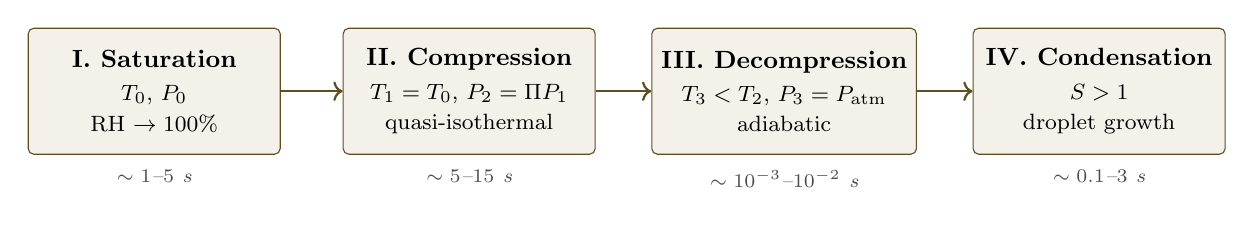
\begin{tikzpicture}[scale=1.0, every node/.style={font=\small}]
  % stage boxes
  \node[draw=accent!70!black, fill=accent!10, rounded corners=2pt, minimum width=3.2cm, minimum height=1.6cm, align=center] (s1) at (0,0) {\textbf{I. Saturation}\\[1pt]\footnotesize $T_0$, $P_0$\\\footnotesize RH $\to 100\%$};
  \node[draw=accent!70!black, fill=accent!10, rounded corners=2pt, minimum width=3.2cm, minimum height=1.6cm, align=center] (s2) at (4,0) {\textbf{II. Compression}\\[1pt]\footnotesize $T_1 = T_0$, $P_2 = \Pi P_1$\\\footnotesize quasi-isothermal};
  \node[draw=accent!70!black, fill=accent!10, rounded corners=2pt, minimum width=3.2cm, minimum height=1.6cm, align=center] (s3) at (8,0) {\textbf{III. Decompression}\\[1pt]\footnotesize $T_3 < T_2$, $P_3 = P_{\text{atm}}$\\\footnotesize adiabatic};
  \node[draw=accent!70!black, fill=accent!10, rounded corners=2pt, minimum width=3.2cm, minimum height=1.6cm, align=center] (s4) at (12,0) {\textbf{IV. Condensation}\\[1pt]\footnotesize $S > 1$\\\footnotesize droplet growth};
  % arrows
  \draw[->, thick, accent!70!black] (s1) -- (s2);
  \draw[->, thick, accent!70!black] (s2) -- (s3);
  \draw[->, thick, accent!70!black] (s3) -- (s4);
  % timescales
  \node[below=2pt of s1, font=\scriptsize\itshape, text=gray!60!black] {$\sim 1$--$5$ s};
  \node[below=2pt of s2, font=\scriptsize\itshape, text=gray!60!black] {$\sim 5$--$15$ s};
  \node[below=2pt of s3, font=\scriptsize\itshape, text=gray!60!black] {$\sim 10^{-3}$--$10^{-2}$ s};
  \node[below=2pt of s4, font=\scriptsize\itshape, text=gray!60!black] {$\sim 0.1$--$3$ s};
\end{tikzpicture}
\caption{\label{fig:phases}The four phases of the OADF event, with characteristic timescales. Phases I and II prepare the thermodynamic state; Phase III drives the adiabatic temperature drop; Phase IV produces the visible plume by condensation onto bio-aerosol CCN.}
\end{figure}

% =========================================================================
\section{Mathematical Formalization}
\label{sec:formalization}
% =========================================================================

We now derive a closed-form expression for the post-expansion saturation ratio $S$ in terms of the controllable input parameter $\Pi$ and the initial cavity temperature $T_0$.

\subsection{Temperature after adiabatic decompression}

From Eq.~(\ref{eq:T3}), assuming Phase II ended at $T_2 = T_1 = T_0$ (isothermal compression limit):
\begin{equation}
\label{eq:T3-final}
T_3(\Pi, T_0) = T_0 \cdot \Pi^{-(\gamma-1)/\gamma}.
\end{equation}
The temperature drop is
\begin{equation}
\Delta T = T_0 - T_3 = T_0\left[1 - \Pi^{-(\gamma-1)/\gamma}\right].
\end{equation}

\subsection{Water-vapor partial pressure after expansion}

From Eq.~(\ref{eq:pw3}) and Phase~II saturation $p_{w,2} = \pwsat(T_0)$:
\begin{equation}
\label{eq:pw3-final}
p_{w,3}(\Pi, T_0) = \frac{\pwsat(T_0)}{\Pi}.
\end{equation}

\subsection{Saturation pressure at the post-expansion temperature}

Combining Eqs.~(\ref{eq:T3-final}) and (\ref{eq:ARM}):
\begin{equation}
\label{eq:psat3}
\pwsat(T_3) = \SI{6.1094}{\hecto\pascal} \cdot \exp\!\left(\frac{17.625 \cdot T_{3,C}}{T_{3,C} + 243.04}\right),
\end{equation}
with $T_{3,C} = T_3 - 273.15$.

\subsection{The saturation ratio}

\begin{equation}
\boxed{
\label{eq:S-final}
S(\Pi, T_0) = \frac{p_{w,3}}{\pwsat(T_3)} = \frac{\pwsat(T_0)}{\Pi \cdot \pwsat\!\left(T_0\,\Pi^{-(\gamma-1)/\gamma}\right)}.
}
\end{equation}

\noindent\textbf{Interpretation.} The compression ratio $\Pi$ enters Eq.~(\ref{eq:S-final}) in two competing ways: through the linear depression of $p_{w,3}$ (denominator factor $\Pi$), and through the exponential depression of $\pwsat(T_3)$ via cooling (the denominator's evaluation of $\pwsat$ at the lower temperature). The exponential dependence of $\pwsat$ on $T$ overwhelms the linear $\Pi$ factor for any $\Pi > 1$, producing $S > 1$. This is the formal reason that even mild compressions produce visible fog: the Clausius–Clapeyron exponential beats the ideal-gas linear scaling.

\subsection{Clausius–Clapeyron derivation of the exponential}

The exponential temperature-dependence of $\pwsat$ that drives the asymmetry above derives from the Clausius–Clapeyron equation \citep{Atkins2010}:
\begin{equation}
\frac{d\pwsat}{dT} = \frac{L_v \pwsat}{R_v T^2},
\end{equation}
where $L_v = \SI{2.45e6}{\joule\per\kilogram}$ is the specific latent heat of vaporization (at \SI{293}{\kelvin}) and $R_v = R/M_w = \SI{461.5}{\joule\per\kilogram\per\kelvin}$. Treating $L_v$ as constant over the relevant temperature range, integration gives
\begin{equation}
\label{eq:CC-integrated}
\pwsat(T) = \pwsat(\Tref)\exp\!\left[\frac{L_v}{R_v}\left(\frac{1}{\Tref} - \frac{1}{T}\right)\right].
\end{equation}
The August–Roche–Magnus form (\ref{eq:ARM}) is an empirical refinement allowing for the modest temperature-dependence of $L_v$. For temperature variations of $\Delta T \lesssim \SI{20}{\kelvin}$, the two forms agree to within $\lesssim 1\%$.

\subsection{Condensable water mass}

The mass of water that must condense per unit volume of plume gas to bring the system back to saturation is
\begin{equation}
\label{eq:dm}
\Delta\rho_w(\Pi, T_0) = \frac{p_{w,3} - \pwsat(T_3)}{R_v T_3} = \frac{\pwsat(T_3)(S-1)}{R_v T_3}.
\end{equation}
This is the excess vapor mass per cubic meter, and serves as the source for droplet growth.

\subsection{Droplet growth and number density}

\subsubsection{Maxwell vapor-diffusion growth}
\label{sec:growth}

An activated droplet of radius $r$ in a supersaturated environment grows by vapor diffusion according to the Maxwell equation \citep{PruppacherKlett2010}:
\begin{equation}
\label{eq:maxwell}
r\frac{dr}{dt} = \frac{D_{w,\text{air}} M_w (\rho_{w,\infty} - \rho_{w,s})}{\rho_w R T},
\end{equation}
which, neglecting Kelvin and Raoult corrections (valid for $r \gg A$), simplifies to the standard form
\begin{equation}
\label{eq:r-grow}
r^2(t) = r_0^2 + 2\xi t, \qquad \xi \equiv \frac{D_{w,\text{air}} \pwsat(T)(S-1)}{\rho_w R_v T}.
\end{equation}
For $T = \SI{302}{\kelvin}$, $\pwsat(T) \approx \SI{3.9}{\kilo\pascal}$, $D_{w,\text{air}} \approx \SI{2.5e-5}{m^2/s}$, $S - 1 = 0.46$, $\rho_w = \SI{e3}{\kilo\gram\per\cubic\meter}$:
\begin{equation}
\xi \approx \frac{(2.5\times 10^{-5})(3.9\times 10^3)(0.46)}{(10^3)(461.5)(302)} \approx \SI{3.2e-10}{m^2/s}.
\end{equation}
A droplet of initial radius $r_0 = \SI{0.1}{\micro\meter}$ grows to $r \approx \SI{1}{\micro\meter}$ in
\begin{equation}
t = \frac{r^2 - r_0^2}{2\xi} \approx \frac{(10^{-6})^2}{2 \cdot 3.2 \times 10^{-10}} \approx \SI{1.6}{\milli\second}.
\end{equation}
This timescale is short compared with the plume dissipation time of $\sim\!\SI{1}{\second}$, confirming that the visible plume is essentially fully developed within the first few milliseconds after lip opening.

\subsubsection{Droplet number density}
The number density of activated droplets is, to leading order,
\begin{equation}
n_d \approx \int_{S_c < S} n_{\text{CCN}}(D)\, dD,
\end{equation}
where $n_{\text{CCN}}(D)$ is the CCN size distribution. For an in-cavity CCN concentration of $\sim\!\SI{e9}{\per\cubic\meter}$ (Sec.~\ref{sec:CCN}) and a supersaturation $S \approx 1.46$ well above the critical supersaturation of typical \SIrange{50}{500}{\nano\meter} dry-radius bio-aerosols ($S_c - 1 \lesssim 0.01$), essentially all CCN are activated. We therefore take
\begin{equation}
n_d \approx n_{\text{CCN}} \sim \SI{e9}{\per\cubic\meter} = \SI{e3}{\per\cubic\centi\meter}.
\end{equation}

\subsubsection{Final droplet radius from mass conservation}

Conservation of condensed water mass gives
\begin{equation}
\label{eq:rfinal}
r_f = \left(\frac{3 \Delta\rho_w}{4\pi \rho_w n_d}\right)^{1/3}.
\end{equation}
For $\Delta\rho_w \approx \SI{12.9}{\gram\per\cubic\meter}$ (Sec.~\ref{sec:numerics}) and $n_d \sim \SI{e9}{\per\cubic\meter}$:
\begin{equation}
r_f \approx \left(\frac{3 \cdot 1.29 \times 10^{-2}}{4\pi \cdot 10^3 \cdot 10^9}\right)^{1/3} \approx \SI{1.45}{\micro\meter}.
\end{equation}
The plume thus consists of $\sim\!\SI{e9}{\per\cubic\meter}$ droplets of radius $\sim\!\SI{1.5}{\micro\meter}$, consistent with Mie-scattering wavelengths and explaining the optical opacity of the visible plume in the visible band ($\lambda \approx \SIrange{400}{700}{\nano\meter}$).

% =========================================================================
\section{Numerical Estimation}
\label{sec:numerics}
% =========================================================================

We now collect the formalism above into a single worked numerical example using physiologically representative parameters.

\subsection{Input parameters}

\begin{table}[h]
\centering
\small
\caption{\label{tab:inputs}Input parameters for the worked numerical estimation.}
\begin{tabular}{@{}llll@{}}
\toprule
\textbf{Symbol} & \textbf{Quantity} & \textbf{Value} & \textbf{Source} \\
\midrule
$T_0$    & Initial buccal temperature   & \SI{310}{\kelvin}              & Body temperature \\
$P_0$    & Atmospheric pressure         & \SI{101.325}{\kilo\pascal}     & Standard \\
$V_0$    & Initial cavity volume        & \SI{100}{\milli\liter}         & \citep{Proctor1977} \\
$\Pi$    & Compression ratio            & 1.10                            & \citep{Hixon1988} \\
$\gamma$ & Heat capacity ratio of air   & 1.40                            & Standard \\
$\mathrm{RH}_0$ & Initial relative humidity & 1.00                       & Sec.~\ref{sec:humidity} \\
$n_{\text{CCN}}$ & In-cavity CCN density & \SI{e9}{\per\cubic\meter}     & Sec.~\ref{sec:CCN} \\
\bottomrule
\end{tabular}
\end{table}

\subsection{Step-by-step calculation}

\paragraph{(a) Saturation vapor pressure at $T_0$.}
From Eq.~(\ref{eq:ARM}) with $T_C = \SI{37}{\celsius}$:
\[
\pwsat(310\,\mathrm{K}) = 6.1094\,\mathrm{hPa} \cdot \exp\!\left(\frac{17.625 \cdot 37}{37 + 243.04}\right) = \SI{62.74}{\hecto\pascal} = \SI{6.274}{\kilo\pascal}.
\]

\paragraph{(b) Pressure after compression.}
\[
P_2 = \Pi \cdot P_0 = 1.10 \cdot 101.325 = \SI{111.46}{\kilo\pascal}.
\]
Water-vapor partial pressure at end of Phase II (isothermal limit): $p_{w,2} = \SI{6.274}{\kilo\pascal}$.

\paragraph{(c) Temperature after adiabatic decompression.}
From Eq.~(\ref{eq:T3-final}):
\[
T_3 = 310 \cdot (1.10)^{-(0.4/1.4)} = 310 \cdot (1.10)^{-0.2857} = 310 \cdot 0.9732 = \SI{301.7}{\kelvin}.
\]
Equivalently, $T_{3,C} = \SI{28.6}{\celsius}$. Temperature drop: $\Delta T = \SI{8.4}{\kelvin}$.

\paragraph{(d) Water-vapor partial pressure after decompression.}
From Eq.~(\ref{eq:pw3-final}):
\[
p_{w,3} = \frac{6.274}{1.10} = \SI{5.704}{\kilo\pascal}.
\]

\paragraph{(e) Saturation pressure at $T_3$.}
From Eq.~(\ref{eq:ARM}) at $T_C = \SI{28.6}{\celsius}$:
\[
\pwsat(T_3) = 6.1094 \cdot \exp\!\left(\frac{17.625 \cdot 28.6}{28.6 + 243.04}\right) = \SI{39.08}{\hecto\pascal} = \SI{3.908}{\kilo\pascal}.
\]

\paragraph{(f) Saturation ratio.}
From Eq.~(\ref{eq:S-final}):
\[
S = \frac{p_{w,3}}{\pwsat(T_3)} = \frac{5.704}{3.908} = 1.460.
\]
The supersaturation is $s = S - 1 = 0.460$, i.e., \SI{46}{\percent}.

\paragraph{(g) Excess water mass per cubic meter.}
From Eq.~(\ref{eq:dm}):
\[
\Delta\rho_w = \frac{(p_{w,3} - \pwsat(T_3))}{R_v T_3} = \frac{(5704 - 3908)}{461.5 \cdot 301.7} = \SI{1.290e-2}{\kilo\gram\per\cubic\meter} = \SI{12.90}{\gram\per\cubic\meter}.
\]

\paragraph{(h) Total condensed mass in expelled plume.}
Volume of expelled gas (post-expansion):
\[
V_3 = V_0 \cdot \Pi^{1/\gamma} \approx 100 \cdot (1.10)^{0.714} = \SI{107.1}{\milli\liter}.
\]
Total condensed water mass:
\[
m_w = \Delta\rho_w \cdot V_3 = 1.29 \times 10^{-2} \cdot 1.071 \times 10^{-4} \approx \SI{1.38}{\milli\gram}.
\]

\paragraph{(i) Final droplet radius (mass-conserved).}
\[
r_f = \left(\frac{3 \cdot 1.29 \times 10^{-2}}{4\pi \cdot 10^3 \cdot 10^9}\right)^{1/3} \approx \SI{1.45}{\micro\meter}.
\]

\paragraph{(j) Mie-scattering visibility.}
The size parameter $x = 2\pi r/\lambda$ at $\lambda = \SI{550}{\nano\meter}$ is $x = 2\pi \cdot 1.45/0.55 \approx 16.6$, placing the droplet firmly in the geometric-optics regime where scattering efficiency $Q_{\text{ext}} \to 2$. Optical opacity is therefore expected for plume thicknesses such that $\tau_{\text{opt}} = n_d \pi r^2 \cdot Q_{\text{ext}} \cdot L \gtrsim 1$, giving $L \gtrsim \SI{0.7}{\centi\meter}$ — easily satisfied by a few-centimeter plume. The plume is predicted to be optically opaque, in agreement with everyday observation.

\subsection{Sensitivity analysis}

The key result $S(\Pi)$ is plotted in Fig.~\ref{fig:Splot} as a function of compression ratio. Inspection shows that even modest compressions ($\Pi \gtrsim 1.05$) generate supersaturations well above the activation thresholds of typical saliva-derived CCN, robustly accounting for the observed phenomenon. Conversely, $\Pi \lesssim 1.02$ yields $S \lesssim 1.05$, below the threshold for visible plume formation.

\begin{figure}[h]
\centering
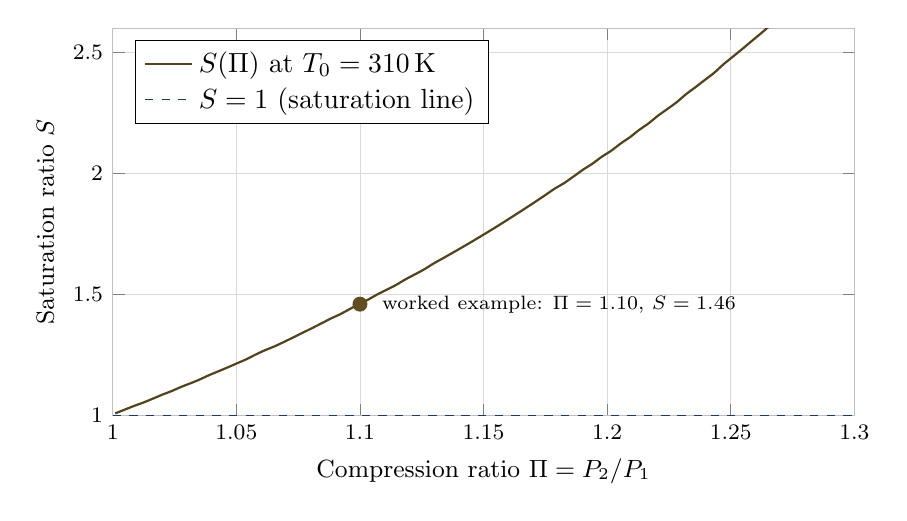
\begin{tikzpicture}
\begin{axis}[
  width=11cm, height=6.5cm,
  xlabel={Compression ratio $\Pi = P_2/P_1$},
  ylabel={Saturation ratio $S$},
  xmin=1.00, xmax=1.30,
  ymin=1.00, ymax=2.6,
  grid=both,
  major grid style={line width=.2pt,draw=gray!30},
  minor grid style={line width=.1pt,draw=gray!15},
  axis line style={draw=gray!50},
  tick label style={font=\footnotesize},
  label style={font=\small},
  legend pos=north west,
  legend cell align=left,
]
% S vs Pi: plotted via samples; T0=310 K; gamma=1.4
\addplot[smooth,thick,color=accent!60!black,samples=80,domain=1.001:1.30]
   ({x}, { (62.74/(x* 6.1094 * exp( 17.625 * (310*x^(-0.2857) - 273.15) / ((310*x^(-0.2857) - 273.15) + 243.04)) )) });
\addplot[dashed,color=linkcolor,domain=1.0:1.3]{1};
\addlegendentry{$S(\Pi)$ at $T_0=\SI{310}{\kelvin}$};
\addlegendentry{$S=1$ (saturation line)};
% mark the worked example
\addplot[only marks,mark=*,mark size=2.5pt,color=accent!70!black] coordinates {(1.10, 1.460)};
\node[anchor=west,font=\scriptsize] at (axis cs:1.105,1.46) {worked example: $\Pi=1.10$, $S=1.46$};
\end{axis}
\end{tikzpicture}
\caption{\label{fig:Splot}Predicted saturation ratio $S$ as a function of compression ratio $\Pi$ at $T_0 = \SI{310}{\kelvin}$, $\gamma = 1.4$ (Eq.~\ref{eq:S-final}). The worked example of Sec.~\ref{sec:numerics} ($\Pi = 1.10$, $S = 1.46$) is marked. The supersaturation threshold $S = 1$ is shown as a dashed line; any $\Pi > 1$ produces supersaturation, with rapid growth above $\Pi \approx 1.05$.}
\end{figure}

\begin{keypoint}[Summary of numerical predictions]
For a representative buccal compression of $\Pi = 1.10$ at $T_0 = \SI{310}{\kelvin}$, the OADF model predicts:
\begin{itemize}
  \item Temperature drop $\Delta T \approx \SI{8.4}{\kelvin}$;
  \item Post-expansion supersaturation $S \approx 1.46$;
  \item Condensable water content $\Delta\rho_w \approx \SI{12.9}{\gram\per\cubic\meter}$;
  \item Total condensed mass per puff $m_w \approx \SI{1.4}{\milli\gram}$;
  \item Droplet number density $n_d \sim \SI{e9}{\per\cubic\meter}$;
  \item Final droplet radius $r_f \approx \SI{1.5}{\micro\meter}$;
  \item Plume optically opaque for thickness $\gtrsim \SI{1}{\centi\meter}$.
\end{itemize}
\end{keypoint}

% =========================================================================
\section{Proposed Experimental Methodology}
\label{sec:experiment}
% =========================================================================

We propose a self-contained experimental protocol to validate the predictions of Sec.~\ref{sec:numerics}.

\subsection{Subjects and ethics}
Healthy adult subjects ($n \ge 10$, balanced for sex, age range 18–45, BMI 18.5–29.9, non-smokers, no oral pathology) recruited under informed consent. Approval from a duly constituted institutional ethics committee is required, even though the maneuver is non-invasive and routine: the protocol involves voluntary intra-oral pressurization comparable to playing a wind instrument, and is low-risk.

\subsection{Instrumentation}

\begin{enumerate}
\item \textbf{Intra-oral pressure transducer.} Catheter-tip transducer (e.g., Millar SPR-524 or equivalent) placed sublingually, bandwidth $\ge \SI{100}{\hertz}$, range $0\text{--}\SI{40}{\kilo\pascal}$, calibrated against a water manometer. Records $P(t)$ during compression and at the moment of decompression.
\item \textbf{Thermometry.} A thin-wire thermocouple (Type K, wire diameter $\le \SI{25}{\micro\meter}$) positioned $\sim\!\SI{2}{\centi\meter}$ outside the lips, in the path of the emerging plume. Response time $\lesssim \SI{10}{\milli\second}$, recorded at $\ge \SI{1}{\kilo\hertz}$.
\item \textbf{Optical particle counter (OPC).} Aerosol size spectrometer (e.g., TSI 3330 or Grimm 11-D) sampling at $\sim\!\SI{1.2}{\liter\per\minute}$ from a Tedlar bag into which the subject deposits the puff. Size range $\SIrange{0.3}{20}{\micro\meter}$, 16-channel.
\item \textbf{High-speed imaging.} Schlieren or shadowgraph setup with a high-speed camera (e.g., Photron Fastcam SA-X, $\ge 5000$~fps) for visualization of plume morphology, expansion velocity, and dissipation time.
\item \textbf{Backlight optical extinction.} A collimated white-light source and photodiode across a known plume thickness for direct measurement of optical density $\tau_{\text{opt}}(t)$.
\end{enumerate}

\subsection{Protocol}

\begin{enumerate}
  \item Subject seated, instrumented with intra-oral pressure transducer, breathing normally for \SI{5}{\minute} to reach baseline oral humidity.
  \item Subject closes lips, performs 10 tongue-palate clicks at $\sim\!\SI{2}{\hertz}$, then applies cheek and Valsalva compression for $\sim\!\SI{3}{\second}$, then releases lips on cue.
  \item Pressure, temperature, and particle size traces synchronized via TTL trigger.
  \item Repeat $\ge 5$ trials per subject with $\ge \SI{2}{\minute}$ recovery between trials.
  \item Control trials: identical maneuver \emph{without} the pre-compression tongue-clicking phase (to assess CCN contribution); and identical maneuver in dehumidified inspired air (to assess humidity contribution).
\end{enumerate}

\subsection{Predicted observable outcomes and falsifiable hypotheses}

\begin{description}
  \item[H1 (central):] Mean intra-oral pressure at release is $\Delta P = \SIrange{5}{15}{\kilo\pascal}$.
  \item[H2:] Mean plume temperature drop is $\Delta T = \SIrange{3}{15}{\kelvin}$, correlated with $\Delta P$ via Eq.~(\ref{eq:T3-final}).
  \item[H3:] Plume droplet count is $\ge \SI{e6}{\per\liter}$ in the post-event Tedlar-bag sample.
  \item[H4:] Plume droplet size distribution peaks at $r \sim \SIrange{0.5}{3}{\micro\meter}$.
  \item[H5 (CCN dependence):] Suppressing the tongue-clicking pre-phase reduces plume optical density by $\ge \SI{50}{\percent}$, while leaving $\Delta T$ approximately unchanged. This isolates the CCN role.
  \item[H6 (humidity dependence):] Dehumidifying inspired air ($\mathrm{RH} \le \SI{20}{\percent}$ for \SI{2}{\minute}) prior to the maneuver eliminates the visible plume entirely, in agreement with the saturation pre-condition.
\end{description}

Failure of H1–H4 within the stated ranges (after correction for instrument response and individual variation) would falsify the central thermodynamic model. Failure of H5 or H6 would falsify the auxiliary microphysical assumptions.

% =========================================================================
\section{Discussion}
\label{sec:discussion}
% =========================================================================

\subsection{Position within the taxonomy of condensation phenomena}
\label{sec:taxonomy}

OADF belongs to a broader family of \emph{expansion-condensation fog} phenomena, distinguished from \emph{mixing fog} phenomena by the source of cooling. Table~\ref{tab:taxonomy} positions OADF among related cases.

\begin{table}[h]
\centering
\footnotesize
\caption{\label{tab:taxonomy}Taxonomy of related condensation phenomena. Decompression-driven phenomena (top) cool the gas by adiabatic expansion. Mixing-driven phenomena (bottom) cool warm humid air by mixing with colder ambient air.}
\begin{tabularx}{\textwidth}{@{}lXll@{}}
\toprule
\textbf{Phenomenon} & \textbf{Mechanism} & \textbf{$\Pi$ or $\Delta T$} & \textbf{CCN source} \\
\midrule
\multicolumn{4}{l}{\emph{Expansion-driven (decompression cooling)}} \\
Wilson cloud chamber                 & Mechanical piston expansion         & $\Pi \sim 1.25\text{--}1.40$ & Designed (ions) \\
Champagne plume                      & Cork ejection from bottleneck       & $\Pi \sim 4\text{--}6$       & CO$_2$ clathrate, dust \\
\textbf{OADF (this work)}            & Buccal lip-release                  & $\Pi \sim 1.05\text{--}1.15$ & Saliva-derived bioaerosol \\
Atmospheric cumulus formation        & Adiabatic rise of air parcel        & $\Pi \sim 1.05\text{--}1.20$ & Dust, salt, sulfate \\
Transonic Prandtl–Glauert cone       & Pressure drop behind shock          & varies                       & Ambient water aerosols \\
\midrule
\multicolumn{4}{l}{\emph{Mixing-driven (radiative or contact cooling)}} \\
Cold-day breath fog                  & Mixing of warm exhalation with cold air & $\Delta T \sim \SI{20}{\kelvin}$ & Saliva-derived bioaerosol \\
Steam-fog over warm water            & Mixing of warm humid air with cold air & varies                    & Ambient \\
Radiation fog                        & Surface cooling by IR emission         & $\Delta T \sim \SIrange{5}{15}{\kelvin}$ & Ambient \\
\bottomrule
\end{tabularx}
\end{table}

\subsection{Distinction from cold-breath fog}
\label{sec:mixingfog}

A common conflation is that OADF and the breath fog visible in cold weather are the same phenomenon. They are not. Cold-breath fog is a \emph{mixing fog}, in which warm exhaled air at $T \approx \SI{310}{\kelvin}$ and $\mathrm{RH} = 100\%$ mixes with cold ambient air at, say, $T_a = \SI{273}{\kelvin}$ and $\mathrm{RH}_a = \SI{50}{\percent}$, producing a transient mixture that briefly exceeds saturation on the mixing line in the $(T, p_w)$ phase plane \citep{Bohren1998}. The mechanism is wholly different: it is the curvature of the saturation curve (Clausius–Clapeyron) that makes the linear mixing line exceed saturation, not the adiabatic decompression that drives OADF. Critically:
\begin{itemize}
  \item Cold-breath fog requires cold ambient air; OADF does not.
  \item OADF requires intra-oral compression; cold-breath fog does not.
  \item OADF is reproducible in a hot, dry room where cold-breath fog is impossible.
\end{itemize}
The phenomena coexist in winter conditions when both mechanisms operate; their decoupling under controlled humidity and temperature conditions provides an additional experimental discriminator.

\subsection{Applications}

\subsubsection{Pedagogical}
OADF offers a zero-cost, ubiquitously available demonstration of adiabatic cooling and supersaturation. It can be performed in any classroom without apparatus, links cleanly to the Wilson cloud chamber's role in particle-physics history, and engages students with a phenomenon they have personally produced. A pedagogical paper deriving Eq.~(\ref{eq:S-final}) from the Poisson and August–Roche–Magnus relations could plausibly find a home in \emph{The Physics Teacher} or \emph{European Journal of Physics}.

\subsubsection{Bioaerosol and respiratory physics}
The droplet population produced by OADF is large ($\sim\!\SI{e9}{\per\cubic\meter}$) and dominated by water condensed onto saliva-derived nuclei. As such, OADF is a candidate as a controlled, voluntary, repeatable generator of respiratory bioaerosols whose nucleating cores are biologically relevant — making it potentially useful in the post-pandemic context of respiratory aerosol research \citep{Asadi2019,Bourouiba2020}, where reproducible aerosol generation from human sources is a methodological bottleneck. Whether OADF-generated aerosols are representative of natural respiratory emissions in their composition, viability of any embedded pathogens, and dispersal characteristics remains an open question worthy of empirical study.

\subsubsection{Science communication}
The phenomenon's universal accessibility makes it well suited to science-communication content, particularly visual media. A high-speed Schlieren video of an OADF event, accompanied by the four-phase decomposition of Sec.~\ref{sec:framework}, would constitute a publishable demonstration in the tradition of the YouTube physics-explainer genre.

% =========================================================================
\section{Limitations and Open Questions}
\label{sec:limits}
% =========================================================================

\subsection{Limitations of the present analysis}

The analysis presented here is theoretical and order-of-magnitude. Several simplifications warrant explicit acknowledgement:

\begin{enumerate}
  \item \textbf{Isothermal Phase II assumption.} We model the compression as quasi-isothermal. A fully adiabatic compression would raise $T_2$ by $\sim\!\SI{8}{\kelvin}$ and proportionally increase $\pwsat$ at the end of Phase II, ultimately yielding a slightly larger plume. The true behaviour lies between the two limits. Direct measurement of $T(t)$ during compression would resolve this.
  \item \textbf{Uniform mole-fraction assumption.} We have treated the cavity gas as homogeneous in composition. In reality, water-vapor concentration is highest near the mucosa and lowest in the central cavity, particularly during dynamic compression. The effect on the global $S$ is small but non-zero.
  \item \textbf{Köhler theory simplifications.} We have employed the classical Köhler equation. For organic-dominated CCN with significant surface-active components (a likely description of saliva-derived aerosols), the surface tension $\sigma_w$ in the Kelvin term may be substantially reduced from its pure-water value, lowering $S_c$ further and broadening the activated CCN population \citep{Facchini1999,Sorjamaa2004}.
  \item \textbf{No droplet–droplet interactions.} We have neglected competition between growing droplets for the limited vapor reservoir, which becomes important once droplets approach the radius set by mass conservation (Eq.~\ref{eq:rfinal}). For the present order-of-magnitude estimates, this is adequate; for quantitative comparison with experiment, the full parcel-model treatment of \citet{Pinsky2013} would be required.
  \item \textbf{Ambient-air mixing during plume dispersion.} The visible-plume lifetime is set in practice by turbulent mixing with unsaturated ambient air rather than by intrinsic droplet kinetics. The mixing dynamics are outside the scope of this paper.
\end{enumerate}

\subsection{Open empirical questions}

\begin{enumerate}
  \item What is the actual intra-oral pressure profile $P(t)$ during a typical OADF maneuver, and how does it vary with subject training, dental anatomy, and clicking technique?
  \item What is the saliva-derived bioaerosol size distribution and chemical composition at the moment of decompression, before condensation begins?
  \item Do OADF-generated droplets contain culturable oral microflora (\textit{Streptococcus mitis}, \textit{S. salivarius}, etc.), and if so at what number density per droplet? The clinical relevance for transmission studies is unclear but plausible.
  \item Is there a measurable individual-variation factor that correlates with subjective ``ease'' of producing the puff? Possible candidates: oral salivary flow rate, lip-seal pressure, palatal arch geometry, tongue mass.
  \item Does the phenomenon show any age dependence? Anecdotal evidence suggests children produce the effect more readily than adults; whether this reflects physiology, technique, or selection bias is unknown.
\end{enumerate}

% =========================================================================
\section{Conclusion}
\label{sec:conclusion}
% =========================================================================

We have provided what we believe is the first dedicated theoretical treatment of a familiar but undocumented phenomenon: the visible white plume produced upon rapid decompression of the moist, voluntarily-pressurized human buccal cavity. The phenomenon, here proposed as \emph{Oral Adiabatic Decompression Fog} (OADF), is shown to be a low-cost, biologically self-sufficient instance of the same physics that underpins the Wilson expansion cloud chamber, the champagne-cork plume, and the formation of atmospheric clouds. The mathematical model — built from the Poisson adiabatic relation, the Clausius–Clapeyron equation, and Köhler theory — yields a closed-form expression for the post-decompression supersaturation (Eq.~\ref{eq:S-final}) and quantitative predictions, summarized in the keypoint of Sec.~\ref{sec:numerics}, that are within reach of any modestly equipped aerosol or respiratory laboratory.

The phenomenon is not new physics. Its claim on the literature rests on (i) the recognition that it has not, to our knowledge, been formally described; (ii) the elegance with which it instantiates classical Wilson-chamber physics with zero apparatus; and (iii) its potential utility in physics pedagogy and in studies of respiratory bioaerosol generation. We hope the proposed nomenclature, the four-phase decomposition, and the closed-form supersaturation relation prove useful starting points for further work, whether experimental, pedagogical, or simply curious.

\medskip
\begin{flushright}
\itshape
``Most of the universe is made of dark matter, dark energy, and ordinary things that nobody has bothered to write down. The first two are hard. The third is easy and worth doing.''
\end{flushright}

% =========================================================================
\section*{Acknowledgments}
% =========================================================================

The author acknowledges helpful discussions with the AI assistant Claude (Anthropic) regarding the formulation of the four-phase decomposition and the literature survey. The model is the author's; any errors are the author's alone.

% =========================================================================
%   REFERENCES (manual thebibliography for portability)
% =========================================================================

\begin{thebibliography}{99}
\small

\bibitem[Asadi et al.(2019)]{Asadi2019}
Asadi, S., Wexler, A.~S., Cappa, C.~D., Barreda, S., Bouvier, N.~M., \& Ristenpart, W.~D. (2019).
Aerosol emission and superemission during human speech increase with voice loudness.
\textit{Scientific Reports}, \textbf{9}(1), 2348.

\bibitem[Atkins \& de Paula(2010)]{Atkins2010}
Atkins, P., \& de Paula, J. (2010).
\textit{Physical Chemistry} (9th ed.).
Oxford University Press.

\bibitem[Bohren \& Albrecht(1998)]{Bohren1998}
Bohren, C.~F., \& Albrecht, B.~A. (1998).
\textit{Atmospheric Thermodynamics}.
Oxford University Press.

\bibitem[Bourouiba(2020)]{Bourouiba2020}
Bourouiba, L. (2020).
Turbulent gas clouds and respiratory pathogen emissions: Potential implications for reducing transmission of COVID-19.
\textit{JAMA}, \textbf{323}(18), 1837--1838.

\bibitem[Callen(1985)]{Callen1985}
Callen, H.~B. (1985).
\textit{Thermodynamics and an Introduction to Thermostatistics} (2nd ed.).
John Wiley \& Sons.

\bibitem[Dawes(1972)]{Dawes1972}
Dawes, C. (1972).
Circadian rhythms in human salivary flow rate and composition.
\textit{Journal of Physiology}, \textbf{220}(3), 529--545.

\bibitem[Edwards et al.(2004)]{Edwards2004}
Edwards, D.~A., Man, J.~C., Brand, P., Katstra, J.~P., Sommerer, K., Stone, H.~A., et al. (2004).
Inhaling to mitigate exhaled bioaerosols.
\textit{Proceedings of the National Academy of Sciences USA}, \textbf{101}(50), 17383--17388.

\bibitem[Facchini et al.(1999)]{Facchini1999}
Facchini, M.~C., Mircea, M., Fuzzi, S., \& Charlson, R.~J. (1999).
Cloud albedo enhancement by surface-active organic solutes in growing droplets.
\textit{Nature}, \textbf{401}, 257--259.

\bibitem[Galison(1997)]{Galison1997}
Galison, P. (1997).
\textit{Image and Logic: A Material Culture of Microphysics}.
University of Chicago Press.

\bibitem[Hixon et al.(1988)]{Hixon1988}
Hixon, T.~J., Hawley, J.~L., \& Wilson, K.~J. (1988).
An around-the-house device for the clinical determination of respiratory driving pressure: A note on making simple even simpler.
\textit{Journal of Speech and Hearing Disorders}, \textbf{53}(4), 470--473.

\bibitem[Humphrey \& Williamson(2001)]{Humphrey2001}
Humphrey, S.~P., \& Williamson, R.~T. (2001).
A review of saliva: Normal composition, flow, and function.
\textit{Journal of Prosthetic Dentistry}, \textbf{85}(2), 162--169.

\bibitem[Köhler(1936)]{Koehler1936}
Köhler, H. (1936).
The nucleus in and the growth of hygroscopic droplets.
\textit{Transactions of the Faraday Society}, \textbf{32}, 1152--1161.

\bibitem[Lawrence(2005)]{Lawrence2005}
Lawrence, M.~G. (2005).
The relationship between relative humidity and the dewpoint temperature in moist air: A simple conversion and applications.
\textit{Bulletin of the American Meteorological Society}, \textbf{86}(2), 225--234.

\bibitem[Liger-Belair et al.(2017)]{LigerBelair2017}
Liger-Belair, G., Cordier, D., Honvault, J., \& Cilindre, C. (2017).
Unveiling CO$_2$ heterogeneous freezing plumes during champagne cork popping.
\textit{Scientific Reports}, \textbf{7}, 10938.

\bibitem[Liger-Belair(2019)]{LigerBelair2019}
Liger-Belair, G. (2019).
Effervescence in champagne and sparkling wines: From grape harvest to bubble rise.
\textit{European Physical Journal: Special Topics}, \textbf{226}, 3--116.

\bibitem[Lindsley et al.(2010)]{Lindsley2010}
Lindsley, W.~G., Pearce, T.~A., Hudnall, J.~B., et al. (2010).
Quantity and size distribution of cough-generated aerosol particles produced by influenza patients during and after illness.
\textit{Journal of Occupational and Environmental Hygiene}, \textbf{9}(7), 443--449.

\bibitem[Mariak et al.(1999)]{Mariak1999}
Mariak, Z., White, M.~D., Lewko, J., Lyson, T., \& Piekarski, P. (1999).
Direct cooling of the human brain by heat loss from the upper respiratory tract.
\textit{Journal of Applied Physiology}, \textbf{87}(5), 1609--1613.

\bibitem[Netsell \& Hixon(1976)]{Netsell1976}
Netsell, R., \& Hixon, T.~J. (1976).
A noninvasive method for clinically estimating subglottal air pressure.
\textit{Journal of Speech and Hearing Disorders}, \textbf{43}(3), 326--330.

\bibitem[Nobel Foundation(1927)]{NobelPrize1927}
The Nobel Prize in Physics 1927.
Nobel Foundation, Stockholm.
Retrieved from \url{https://www.nobelprize.org/prizes/physics/1927/}

\bibitem[Papineni \& Rosenthal(1997)]{Papineni1997}
Papineni, R.~S., \& Rosenthal, F.~S. (1997).
The size distribution of droplets in the exhaled breath of healthy human subjects.
\textit{Journal of Aerosol Medicine}, \textbf{10}(2), 105--116.

\bibitem[Pinsky et al.(2013)]{Pinsky2013}
Pinsky, M., Mazin, I.~P., Korolev, A., \& Khain, A. (2013).
Supersaturation and diffusional droplet growth in liquid clouds.
\textit{Journal of the Atmospheric Sciences}, \textbf{70}, 2778--2793.

\bibitem[Proctor(1977)]{Proctor1977}
Proctor, D.~F. (1977).
The upper airways. I. Nasal physiology and defense of the lungs.
\textit{American Review of Respiratory Disease}, \textbf{115}(1), 97--129.

\bibitem[Pruppacher \& Klett(2010)]{PruppacherKlett2010}
Pruppacher, H.~R., \& Klett, J.~D. (2010).
\textit{Microphysics of Clouds and Precipitation} (2nd ed., revised).
Springer.

\bibitem[Reif(1965)]{Reif1965}
Reif, F. (1965).
\textit{Fundamentals of Statistical and Thermal Physics}.
McGraw-Hill.

\bibitem[Rogers \& Yau(1989)]{Rogers1989}
Rogers, R.~R., \& Yau, M.~K. (1989).
\textit{A Short Course in Cloud Physics} (3rd ed.).
Pergamon Press.

\bibitem[Seinfeld \& Pandis(2016)]{SeinfeldPandis2016}
Seinfeld, J.~H., \& Pandis, S.~N. (2016).
\textit{Atmospheric Chemistry and Physics: From Air Pollution to Climate Change} (3rd ed.).
John Wiley \& Sons.

\bibitem[Sorjamaa et al.(2004)]{Sorjamaa2004}
Sorjamaa, R., Svenningsson, B., Raatikainen, T., Henning, S., Bilde, M., \& Laaksonen, A. (2004).
The role of surfactants in Köhler theory reconsidered.
\textit{Atmospheric Chemistry and Physics}, \textbf{4}, 2107--2117.

\bibitem[Vollmer \& Möllmann(2008)]{Vollmer2008}
Vollmer, M., \& Möllmann, K.-P. (2008).
Vapour pressure and adiabatic cooling from champagne: Slow-motion visualization of gas thermodynamics.
\textit{Physics Education}, \textbf{47}(5), 608--615.

\bibitem[Wilson(1897)]{Wilson1897}
Wilson, C.~T.~R. (1897).
Condensation of water vapour in the presence of dust-free air and other gases.
\textit{Philosophical Transactions of the Royal Society A}, \textbf{189}, 265--307.

\bibitem[Wilson(1899)]{Wilson1899}
Wilson, C.~T.~R. (1899).
On the condensation nuclei produced in gases by the action of Röntgen rays, uranium rays, ultra-violet light, and other agents.
\textit{Philosophical Transactions of the Royal Society A}, \textbf{192}, 403--453.

\bibitem[Wilson(1911)]{Wilson1911}
Wilson, C.~T.~R. (1911).
On a method of making visible the paths of ionising particles through a gas.
\textit{Proceedings of the Royal Society A}, \textbf{85}(578), 285--288.

\bibitem[Yang et al.(2007)]{Yang2007}
Yang, S., Lee, G.~W.~M., Chen, C.-M., Wu, C.-C., \& Yu, K.-P. (2007).
The size and concentration of droplets generated by coughing in human subjects.
\textit{Journal of Aerosol Medicine}, \textbf{20}(4), 484--494.

\end{thebibliography}

% =========================================================================
\appendix
% =========================================================================

\section{Symbol Glossary}
\label{app:glossary}

\begin{tabular}{@{}lll@{}}
\toprule
\textbf{Symbol} & \textbf{Quantity} & \textbf{Typical value} \\
\midrule
$T_0$, $T_1$, $T_2$, $T_3$ & Temperatures at end of phases 0, I, II, III & $\sim\SI{300}{}$--$\SI{310}{\kelvin}$ \\
$P_0$, $P_1$, $P_2$, $P_3$ & Pressures at end of phases 0, I, II, III & $\sim\SIrange{100}{115}{\kilo\pascal}$ \\
$V_0$ & Initial buccal cavity volume & $\sim\SI{100}{\milli\liter}$ \\
$\Pi$ & Compression ratio $P_2/P_1$ & $\sim 1.10$ \\
$\gamma$ & Heat capacity ratio of air & $1.40$ \\
$p_w$ & Water-vapor partial pressure & varies \\
$\pwsat(T)$ & Saturation vapor pressure of water at $T$ & \SI{6.27}{\kilo\pascal} at \SI{37}{\celsius} \\
$S$ & Saturation ratio $p_w/\pwsat$ & $\sim 1.46$ \\
$s = S-1$ & Supersaturation & $\sim 0.46$ \\
$\rho_w$ & Density of liquid water & $\SI{e3}{\kilo\gram\per\cubic\meter}$ \\
$\sigma_w$ & Surface tension of water & $\sim\SI{0.072}{\newton\per\meter}$ \\
$M_w$ & Molar mass of water & \SI{18.015}{\gram\per\mole} \\
$R$ & Universal gas constant & \SI{8.314}{\joule\per\mole\per\kelvin} \\
$R_v$ & Specific gas constant for water vapor & \SI{461.5}{\joule\per\kilogram\per\kelvin} \\
$L_v$ & Latent heat of vaporization & $\sim\SI{2.45e6}{\joule\per\kilogram}$ \\
$D_{w,\text{air}}$ & Vapor diffusion coefficient in air & $\sim\SI{2.5e-5}{m^2/s}$ \\
$A$, $B$ & Köhler coefficients (Kelvin, Raoult) & Eq.~(\ref{eq:AB}) \\
$r$ & Droplet radius & $\sim\SI{1.5}{\micro\meter}$ (final) \\
$r_c$, $S_c$ & Köhler critical radius, supersaturation & Eqs.~(\ref{eq:rcrit}), (\ref{eq:Scrit}) \\
$n_{\text{CCN}}$ & Cloud condensation nucleus number density & $\sim\SI{e9}{\per\cubic\meter}$ \\
$n_d$ & Activated droplet number density & $\sim\SI{e9}{\per\cubic\meter}$ \\
$\Delta\rho_w$ & Condensable water mass density & $\sim\SI{12.9}{\gram\per\cubic\meter}$ \\
$m_w$ & Total condensed water per puff & $\sim\SI{1.4}{\milli\gram}$ \\
$\tau_{\text{exp}}$ & Expansion timescale & $\sim\SI{10}{\milli\second}$ \\
$\tau_{\text{th}}$ & Thermal diffusion timescale & $\sim\SI{4.5}{\second}$ \\
$Q_{\text{ext}}$ & Mie extinction efficiency & $\to 2$ (geometric regime) \\
$\tau_{\text{opt}}$ & Optical depth of plume & $\gtrsim 1$ for $L \gtrsim \SI{1}{\centi\meter}$ \\
\bottomrule
\end{tabular}

\section{Detailed derivation of the supersaturation relation}
\label{app:derivation}

We here derive Eq.~(\ref{eq:S-final}) explicitly.

\paragraph{Step 1: Adiabatic temperature change.}
Starting from the Poisson relation $TP^{(1-\gamma)/\gamma} = \text{const}$ applied between Phase~II end (state 2) and Phase~III end (state 3):
\begin{equation*}
T_2 P_2^{(1-\gamma)/\gamma} = T_3 P_3^{(1-\gamma)/\gamma},
\end{equation*}
yielding
\begin{equation*}
T_3 = T_2 \left(\frac{P_2}{P_3}\right)^{(1-\gamma)/\gamma} = T_2 \left(\frac{P_3}{P_2}\right)^{(\gamma-1)/\gamma}.
\end{equation*}
With $P_3/P_2 = 1/\Pi$ and the isothermal Phase~II ($T_2 = T_0$):
\begin{equation*}
T_3 = T_0 \cdot \Pi^{-(\gamma-1)/\gamma}.
\end{equation*}
\hfill (Eq.~\ref{eq:T3-final})

\paragraph{Step 2: Adiabatic partial-pressure change.}
For an ideal-gas mixture undergoing adiabatic expansion with conserved mole fractions, each component obeys
\begin{equation*}
p_i V^\gamma = \text{const}.
\end{equation*}
Hence, for the water-vapor component,
\begin{equation*}
\frac{p_{w,3}}{p_{w,2}} = \left(\frac{V_2}{V_3}\right)^\gamma = \left(\frac{P_3}{P_2}\right) = \frac{1}{\Pi},
\end{equation*}
where the last equality uses $PV^\gamma = \text{const}$ for the total mixture. Thus
\begin{equation*}
p_{w,3} = \frac{p_{w,2}}{\Pi} = \frac{\pwsat(T_0)}{\Pi}.
\end{equation*}
\hfill (Eq.~\ref{eq:pw3-final})

\paragraph{Step 3: Saturation ratio.}
By definition,
\begin{equation*}
S = \frac{p_{w,3}}{\pwsat(T_3)} = \frac{\pwsat(T_0)/\Pi}{\pwsat(T_0 \cdot \Pi^{-(\gamma-1)/\gamma})}.
\end{equation*}
Rearranging gives Eq.~(\ref{eq:S-final}). $\qed$

\paragraph{Step 4: Asymptotic regimes.}
For $\Pi \to 1^+$, expand $\Pi = 1 + \epsilon$ with $\epsilon \ll 1$:
\begin{align*}
T_3 &\approx T_0\left[1 - \frac{\gamma-1}{\gamma}\epsilon + O(\epsilon^2)\right], \\
\Delta T &\approx \frac{\gamma-1}{\gamma} T_0 \epsilon \approx 0.286 \cdot T_0 \cdot \epsilon.
\end{align*}
Using the Clausius–Clapeyron equation,
\begin{equation*}
\frac{\pwsat(T_3)}{\pwsat(T_0)} \approx 1 - \frac{L_v}{R_v T_0^2}\Delta T = 1 - \frac{L_v(\gamma-1)\epsilon}{\gamma R_v T_0},
\end{equation*}
so
\begin{equation*}
S \approx \frac{1}{1+\epsilon} \cdot \frac{1}{1 - L_v(\gamma-1)\epsilon/(\gamma R_v T_0)} \approx 1 + \left[\frac{L_v(\gamma-1)}{\gamma R_v T_0} - 1\right]\epsilon + O(\epsilon^2).
\end{equation*}
Inserting numerical values at $T_0 = \SI{310}{\kelvin}$: $L_v(\gamma-1)/(\gamma R_v T_0) = (2.45\times10^6 \cdot 0.4)/(1.4 \cdot 461.5 \cdot 310) \approx 4.89$.
Therefore $S - 1 \approx 3.89 \cdot \epsilon$, indicating that supersaturation grows nearly four times faster than the compression ratio for small $\epsilon$. A \SI{10}{\percent} compression ($\epsilon = 0.10$) yields $S - 1 \approx 0.39$, in good agreement with the exact value $0.46$ computed in Sec.~\ref{sec:numerics}. The factor $\sim 4$ amplification is the formal expression of the everyday observation that the OADF plume is surprisingly robust for such modest pressure differences.

\end{document}
